\documentclass[a4paper,12pt]{article} 

% packages and main settings
\usepackage[left=3cm, right=2cm, top=2cm, bottom=2cm]{geometry}
\usepackage[english]{babel}    
\usepackage[utf8]{inputenc}  
\usepackage[T1]{fontenc}        
\usepackage{lmodern}            
\usepackage{microtype}          
\usepackage{amsmath}
\usepackage{amsfonts, amsthm, amssymb, graphicx, booktabs}
\usepackage{bm} %bold epsilon
\usepackage{newclude}   
\usepackage{placeins}  %surpresses floating tables
\usepackage[labelfont=bf]{caption} %Figure etc steht dann in small caps 
\usepackage[labelsep=period]{caption} % dot after figure, table caption.
\usepackage[flushleft]{threeparttable} % for notes below table
\usepackage{multirow} % for table cell merge along rows
\usepackage{graphicx} % to adjust tablesize to textwidth
\usepackage{caption}  % for centered captions
\usepackage{float} % to set of autopositioning of tables
\usepackage[bottom,hang,flushmargin]{footmisc} % forces footnotes to the bottom
\usepackage{setspace}           % Fuer 1.5 fachen Zeilenabstand  
\onehalfspacing % 1.5 cm Zeilenabstand
%Bibtex
\usepackage[round,sort&compress]{natbib}

\bibliographystyle{chicago} % chicago bib style like in AER
\usepackage[hidelinks]{hyperref} % fuer links und verweise. Cleverref ist eigentlich besser. 


% Create header. The header must be surpressed for 
% every first page per section and a solution
% for the Appendix is used in the respective subfile.
\usepackage{fancyhdr}
\pagestyle{fancy}
\fancyhf{}
\chead{\nouppercase{\textit{\leftmark}}}
\cfoot{\thepage}
\renewcommand{\headrulewidth}{0pt} % no vertical line

%\usepackage{lipsum}  % check if formats work

\usepackage{afterpage} %clearpage w/o pagebreak for "header bug"

% Expectation symbol
\DeclareMathOperator*{\E}{\mathbb{E}}

% thin space, limits underneath in displays
% for strike through
\DeclareMathOperator*{\argmax}{argmax}
\newcommand*{\defeq}{\stackrel{\text{def}}{=}}
\usepackage[normalem]{ulem}
% try to use strikeout in section headers and others
\DeclareRobustCommand{\hsout}[1]{\texorpdfstring{\sout{#1}}{#1}}

% for gray table row color
\usepackage[table]{xcolor}

% decimal dot alignment in table columns
\usepackage{siunitx}

% for footnotes in table
\usepackage[flushleft]{threeparttable}

% for underbar
\newcommand{\ubar}[1]{\text{\b{$#1$}}}

\usepackage{tikz}

% Setup for urls
\usepackage{url}

\defcitealias{Respy-Stenzel.2019}{\textit{respy}}
\defcitealias{Gabler.2019}{\textit{estimagic}}
\defcitealias{Stenzel.2020}{\textit{Master's Thesis Replication Repository}}
\defcitealias{NLSY79}{NLSY79}


\usepackage{tikz}
\begin{document}

\newpage % delete after section is complete

\section{Results}

The section is divided in two parts. First, I present the results of the uncertainty analysis for an overview of the general variation in QoI $Y$. Thereafter, I present the results of the qualitative GSA. The aim is to draw inferences about the contribution of an individual input $X_i$ and its uncertainty on the uncertainty in QoI $Y$ to a degree that allows the identification of non-influential parameters.

\subsection{Uncertainty Analysis}
The following results are obtained by evaluating the occupational choice model at each parameter vector from a random sample. This sample is drawn from the estimated joint distribution. The number of draws is $10,000$. A reasonable level of convergence has already been achieved after about 800 evaluation.\footnote{See the respective notebook in the \citetalias{Stenzel.2020}.}


Figure \ref{fig:uq_paths} incorporates the input uncertainty in the shares of life-time occupation decisions that we have previously seen in Figure \ref{fig:paths}. It depicts the mean and the intervals for $99\%$ of the shares' probability distribution. We can see that the input uncertainty has an effect on the decisions for white- and blue-collar occupation but almost none on the decision for occupation in the education and home sector. This suggests that individuals mainly tend to change between occupation in blue- and white-collar occupation given the distribution of input parameters. Yet, the uncertainty in the shares for both labour sectors is not strikingly large. There is also no visible difference in the uncertainties between both scenarios.
\begin{figure}[H]
	\caption{Comparison of shares of occupation decision over time between scenarios including 99$\%$ confidence intervals}
	\centering
	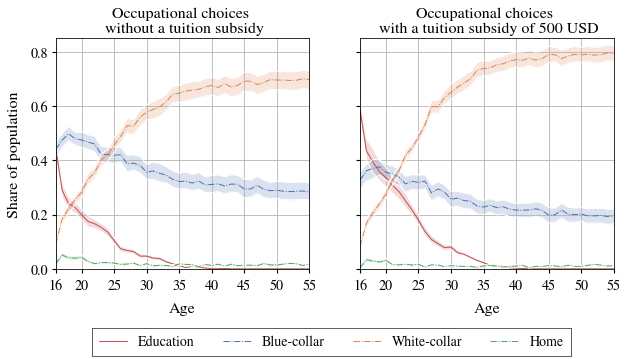
\includegraphics[scale=0.75]{../../../scrypy/figures/cone_plot_choice_shares}
	\label{fig:uq_paths}
\end{figure}

\noindent
Figure \ref{fig:dist} shows the probability distribution for QoI $Y$. The colorised bars depict the realisations within one and two and outside of two standard deviations, $\sigma_Y$, from sample mean $\overline{Y}$.  The distribution is minimally skewed to the left but can be considered as almost normal. This leads to the first conclusion for a potential quantitative GSA. That is, variance-based measures like Sobol' indices can be used because the variance is a good summary measure for normally distributed random variables.

Standard deviation $\sigma_Y$ equals 0.1 and variance $\sigma_Y^2$ equals 0.01. The final goal of a quantitative GSA is to compute the share that input parameter $X_i$ and its variation contribute to $\sigma_Y$ or $\sigma_Y^2$. We can expect that reasonable measures for the contribution of $X_i$ are not completely detached from the measures for the total variation in $Y$ if they are on the same scale. As we have seen earlier, for a linear function without interactions and correlations, we would even expect that the contribution of $X_i$ are smaller than the measure for the variation in $Y$.

The next section computes measures for these contributions.\footnote{For QoI $Y$, it is not necessary to compute the probabilities for specific regions in the probability space of $Y$. The reasons is that, for example in contrary to models for nuclear power plants, there are no regions that are particularly critical.}
\begin{figure}[H]
	\caption{Probability distribution of quantity of interest $q$}
	\centering
	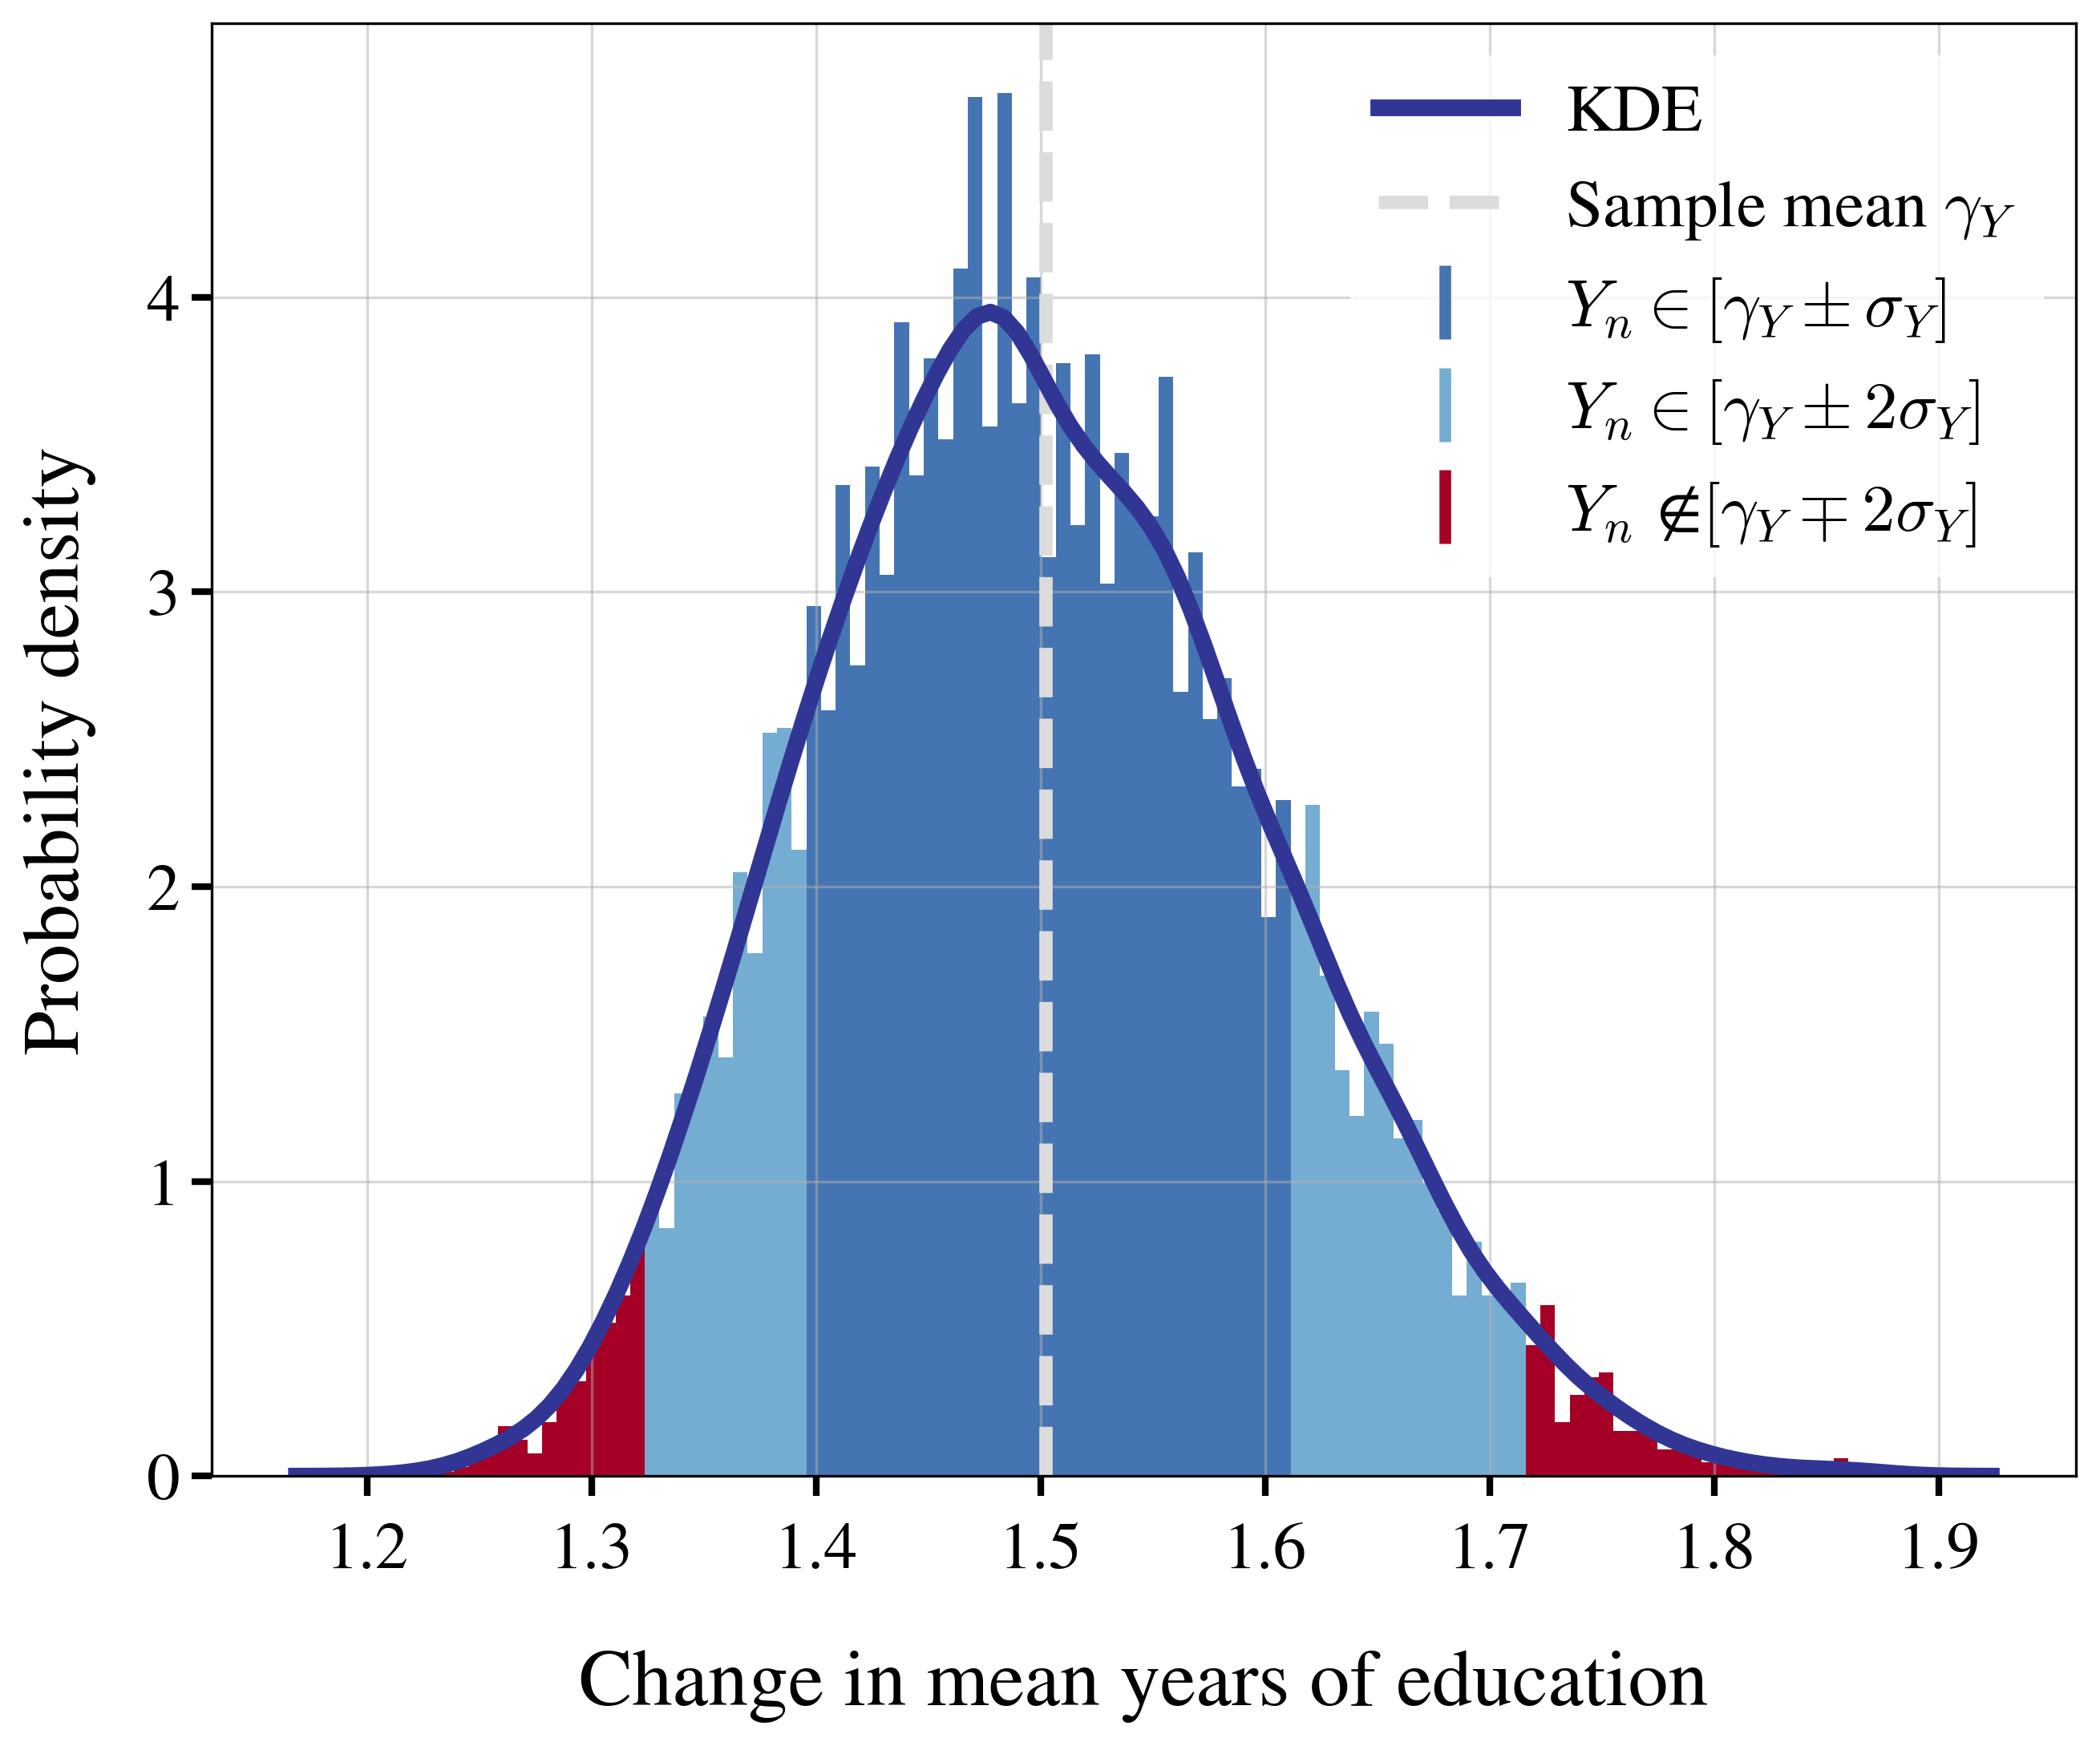
\includegraphics[scale=0.5]{../../../scrypy/figures/distplot}
	\label{fig:dist}
\end{figure}


\newpage
\subsection{Quantitative Global Sensitivity Analysis}
The analysis is divided in three parts. The first part computes the measures by \cite{ge2017extending} for the occupational choice model to validate the conceptual analysis and the results derived from the linear test function. The second part computes measures based on the further developed EEs. They are used for a comparison with the first part and also to compare the two sampling schemes. The third part presents results for a measure that combines the influence of $X_i$ on the level and on the variation of QoI $Y$. This measure is used for cautious recommendation about which input parameters are rather non-influential.

Due to time restrictions, I am only able to present results based on 100 samples in trajectory and radial designs. This is equal to 8200 and 8100 model evaluations.\\

\noindent
Table \ref{tab:kw94gm17} presents the aggregate measures for the full and independent EEs as developed in \cite{ge2014efficient}. I choose the trajectory design because it does not produce extreme steps $b-a$. Additionally I have more control over the set of random parameters and can adjust it to the relatively low number of draws for the subsamples. The numerical parameters that I use are numeric zero, $0^{num}$, equals 0.005 and number of grid points in [0,1], $l$, equals 100. The 100 trajectories are selected based on 200 trajectories in standard normal space following the first improvement in \cite{ge2014efficient}. I do not use the unit space for the post-selection because I do not want to have a concentration of draws in the centre of the normal space. I use this procedure for all trajectory samples throughout the section.

The second and third columns depict the mean absolute EEs, $\mu^{*,full}_T$ and $\mu^{*,ind}_T$ and the fourth and fifth columns show the standard deviations of the EEs, $\mu^{*,ind}_T$ and $\sigma^{*,full}_T$.The authors state that mean EEs and standard deviations have to be interpreted jointly for inferences about the variance of $Y$. Additionally, if for one parameter $X_i$, the full measures are close to 0, the independent measures must also be low to infer that this parameter can be fixed.

We make the following four main observations. First, the level of mean effects and standard deviations is very similar for each variable. Following the interpretation by \cite{ge2017extending} this would suggest that there are no parameters with low effect on the level but high effect on the variation of $Y$. Second, the highest $\mu^{*,full}$ and $\sigma^{*,full}_T$ are achieved by the coefficients for the quadratic (cross-sector) experience for blue- and white-collar sector, $\beta^b_{bb}$, $\beta^b_{ww}$, $\beta^w_{ww}$, $\beta^w_{bb}$. This makes sense because, first, quadratic terms should dominate linear terms (if the variation is comparable and the level is above for value larger than |1|), and second, Figure \ref{fig:uq_paths} already indicated that the home and the education sector are less important for the variation in $Y$. The third observation is that the $\mu^{*,full}$ and $\sigma^{*,full}_T$ contain large variations amongst the different parameters and very high values. These values seem detached from the level of the variation in $Y$. The fourth observation is that the results for the independent measures all below 0.005. Following \cite{ge2014efficient}, this would mean, that there each parameter with full measures close to zero, i.e. all parameters for the home and the education sector can be fixed as the independent measures are close to zero anyway.\\

\noindent
The third and fourth observation is exactly what is expected from the previous conceptual and practical analyses of the measures in \cite{ge2017extending}. Let us first analyse the fourth observation. The independent Elementary Effects are strongly deflated for parameters with large correlations because the denominator does not account for the second transformation step, that involved the lower Cholesky matrix, $Q^T$, of the correlation matrix. As the correlations between all parameters are relatively high, all parameters, even those for the blue- and white-collar sector, are close to 0. The third observation, extreme values for the full measures, can be explained by the transformations that are also missing in the EEs denominator, namely the transformation from uniform to normal space in Step 1 and Step 3. This non-linear transformation is not equalized and therefore, comparably high values are even higher. Both explanations will be confirmed in the next analysis part by the respective columns for the further developed measures $\mu^{*,full}_T$ and $\mu^{*,ind}_T$ in Table \ref{tab:params}.
\newpage
\setlength{\tabcolsep}{22pt} %from 6
\begin{table}[H] 
	\centering
	\begin{threeparttable}
		\caption[Model Parametrization]{EE-based measures by \cite{ge2017extending} for 100 trajectories}
		\label{tab:kw94gm17}
		\renewcommand{\arraystretch}{1.2}%
		\begin{tabular}{cS[table-format=3.2]S[table-format=3.2]@{\hskip 0.7in}|@{\hskip 0.5in}S[table-format=3.2]S[table-format=3.2]}
			
			{Parameter}     & {$\mu^{*,full}_T$}   & {$\mu^{*,ind}_T$} & {$\sigma^{*,full}_T$} & {$\sigma^{*,ind}_T$}\\ \midrule
			\textit{General} \\
			$\delta$ & 53.40   & 0.00 & 69.23 & 0.09   \\    \midrule
			\textit{Blue-collar}\\    
			$\beta^b$ & 3.55   & 0.05            & 4.38 & 0.07    \\
			$\beta_e^b$ & 39.84  &    0.05        & 49.69  & 0.07    \\
			$\beta^b_b$ & 77.21  & 0.05            & 90.23  & 0.07    \\
			$\beta^b_{bb}$ & 2616.50 & 0.05           & 3357.92  & 0.06     \\
			$\beta^b_w$ & 94.74    & 0.05             & 113.49  &  0.06  \\
			$\beta^b_{ww}$ & 1136.58    & 0.03          & 1405.94 &  0.04    \\ \midrule
			\textit{White-collar}\\
			$\beta^w$ & 5.07   & 0.05            & 6.42 &  0.06   \\
			$\beta^w_e$ & 90.25   & 0.07          & 111.50 &  0.08    \\
			$\beta^w_w$ & 82.88  & 0.05            & 103.66 &  0.07   \\
			$\beta^w_{ww}$ & 2444.13  & 0.06           & 3044.69 & 0.07   \\
			$\beta^w_b$ & 452.91 & 0.07           & 490.31 &  0.09   \\
			$\beta^w_{bb}$ & 4317.58 & 0.05         & 4851.54 &  0.06   \\ \midrule
			\textit{Education} \\
			$\beta^e$     & 0.00    & 0.09             & 0.00&  0.10   \\
			$\beta_{he}^e$     & 0.00    & 0.11              & 0.00  & 0.13    \\
			$\beta_{re}^e$     & 0.00  & 0.04               & 0.000  &   0.09  \\ \midrule
			\textit{Home} \\
			$\beta^h$    & 0.00  & 0.04                 & 0.00  & 0.05     \\ \midrule
			\multicolumn{4}{l}{\textit{Lower Triangular Cholesky Matrix}} \\
			$c_{1}$      & 27.94    & 0.07             & 33.72 &  0.08   \\
			$c_{2}$      & 31.89   & 0.05             & 38.58 & 0.06   \\
			$c_{3}$      & 0.00   & 0.06             & 0.00 & 0.07    \\
			$c_{4}$      & 0.00    & 0.04              & 0.00 & 0.09    \\
			$c_{1,2}$     & 12.41   & 0.06            & 14.33 &  0.08  \\
			$c_{1,3}$      & 0.00   & 0.09              & 0.00 &  0.10   \\
			$c_{2,3}$      & 0.00    & 0.05             &  0.00 &   0.06 \\
			$c_{1,4}$      & 0.00    & 0.04            &   0.00 &  0.05 \\
			$c_{2,4}$      & 0.00    & 0.03           & 0.00  &  0.03  \\
			$c_{3,4}$      & 0.00   & 0.04                & 0.00  &  0.05   \\ \bottomrule
		\end{tabular}
	\end{threeparttable}
\end{table}
\newpage

Table \ref{tab:devees} depict the further developed measures that correspond to the mean absolute relative EEs, $\mu^{*,full}$ and $\mu^{*,ind}$ for both sampling schemes in \cite{ge2017extending}. As in Table \ref{tab:kw94gm17}, the standard deviations, in genera, are relatively close to the Elementary Effects. \\

\noindent
The analysis of Table \ref{tab:devees} is divided in three parts. First, I compare the results in \ref{tab:devees} to the findings in Table \ref{tab:kw94gm17}. Then, I compare the results with respect to the different sampling schemes. Thereafter, I analyse more general findings.\\

\noindent
One observation from Table \ref{tab:kw94gm17} are that $\mu^{*,full_T}$ and $\sigma^{*,full}_T$ have a large variation caused by the unbalanced non-linear transformation in the numerator of the respective EEs. This causes larger values to be even larger. Comparing column $\mu^{*,full}_T$ in Table \ref{tab:kw94gm17} with column $\mu^{*,c}_T$ in Table \ref{tab:devees}, we find that the value are indeed, more compressed. This again confirms the first drawback in \cite{ge2017extending}. Still, the variation in $\mu^{*,c}_T$ is relatively large. One explanation is that the model itself is highly non-linear many input parameters.

Another observation from Table \ref{tab:kw94gm17} is that $\mu^{*,ind}_T$ and $\sigma^{*,ind}_T$ are both close to zero because these respective EEs deflate parameters with larger correlations. Looking at $\mu^{*,c}_T$, we find that this drawback is also erased, such that the correlated and uncorrelated can now, potentially, be interpreted jointly for factor fixing. We also see, that $\mu^{*,u}$ is even larger than $\mu^{*,c}$ for both designs. I discuss this point later.\\

\noindent




\newpage
\setlength{\tabcolsep}{22pt} %from 6
\begin{table}[H] 
	\centering
	\begin{threeparttable}
		\caption[Model Parametrization]{Mean absolute correlated and uncorrelated elementary effects\\ (based on 100 subsamples in trajectory and radial design)}
		\label{tab:devees}
		\renewcommand{\arraystretch}{1.2}%
		\begin{tabular}{cS[table-format=3.2]S[table-format=3.2]@{\hskip 0.7in}|@{\hskip 0.5in}S[table-format=3.2]S[table-format=3.2]}

			{Parameter}     & {$\mu^{*,c}_T$}   & {$\mu^{*,c}_R$} & {$\mu^{*,u}_T$} & {$\mu^{*,u}_R$}\\ \midrule
			\textit{General} \\
			$\delta$ & 17   & 23 & 476 & 415   \\    \midrule
			\textit{Blue-collar}\\    
			$\beta^b$ & 1   & 3            & 43 & 88    \\
			$\beta_e^b$ & 11  &    14        & 406  & 443    \\
			$\beta^b_b$ & 25  & 51            & 688  & 1169    \\
			$\beta^b_{bb}$ & 871 & 934           & 15540  & 17860     \\
			$\beta^b_w$ & 29    & 48             & 73  &  143  \\
			$\beta^b_{ww}$ & 389    & 460           & 869 &  1183    \\ \midrule
			\textit{White-collar}\\
			$\beta^w$ & 1   & 3            & 50 &  117   \\
			$\beta^w_e$ & 26   & 28          & 943 &  852    \\
			$\beta^w_w$ & 24  & 47            & 718 &  1521   \\
			$\beta^w_{ww}$ & 933  & 997           & 12257 & 18069   \\
			$\beta^w_b$ & 131 & 127           & 309 &  356   \\
			$\beta^w_{bb}$ & 1230 & 1352         & 2088 &  2477   \\ \midrule
			\textit{Education} \\
			$\beta^e$     & 0.0008    & 0.0002              & 0.001&  0.003   \\
			$\beta_{he}^e$     & 0.0001    & 0.0002              & 0.001  & 0.001    \\
			$\beta_{re}^e$     & 0.0003   & 0.0002               & 0.0003  &   0.0006  \\ \midrule
			\textit{Home} \\
			$\beta^h$    & 0.0003  & 0.0003                 & 0.00002  & 0.00002     \\ \midrule
			\multicolumn{4}{l}{\textit{Lower Triangular Cholesky Matrix}} \\
			$c_{1}$      & 8    & 16             & 18 &  37   \\
			$c_{2}$      & 8   & 11             & 22 & 24   \\
			$c_{3}$      & 0.0004   & 0.0004             & 0.0004 & 0.0007    \\
			$c_{4}$      & 0.0004    & 0.00008              & 0.0002 & 0.0003    \\
			$c_{1,2}$     & 4   & 4            & 10 &  10  \\
			$c_{1,3}$      & 0.0005   & 0.0006              & 0.0006 &  0.0005   \\
			$c_{2,3}$      & 0.0003    & 0.0005             &  0.0006 &   0.001 \\
			$c_{1,4}$      & 0.00004    & 0.00005            &   0.0004 &  0.0005 \\
			$c_{2,4}$      & 0.0001    & 0.0002           & 0.0001  &  0.0002  \\
			$c_{3,4}$      & 0.0001   & 0.0001                & 0.00008  &  0.0001   \\ \bottomrule
		\end{tabular}
	\end{threeparttable}
\end{table}
\newpage
\begin{figure}[H]
	\caption{Sigma-normalized mean absolute Elementary Effects for trajectory design}
	\centering
	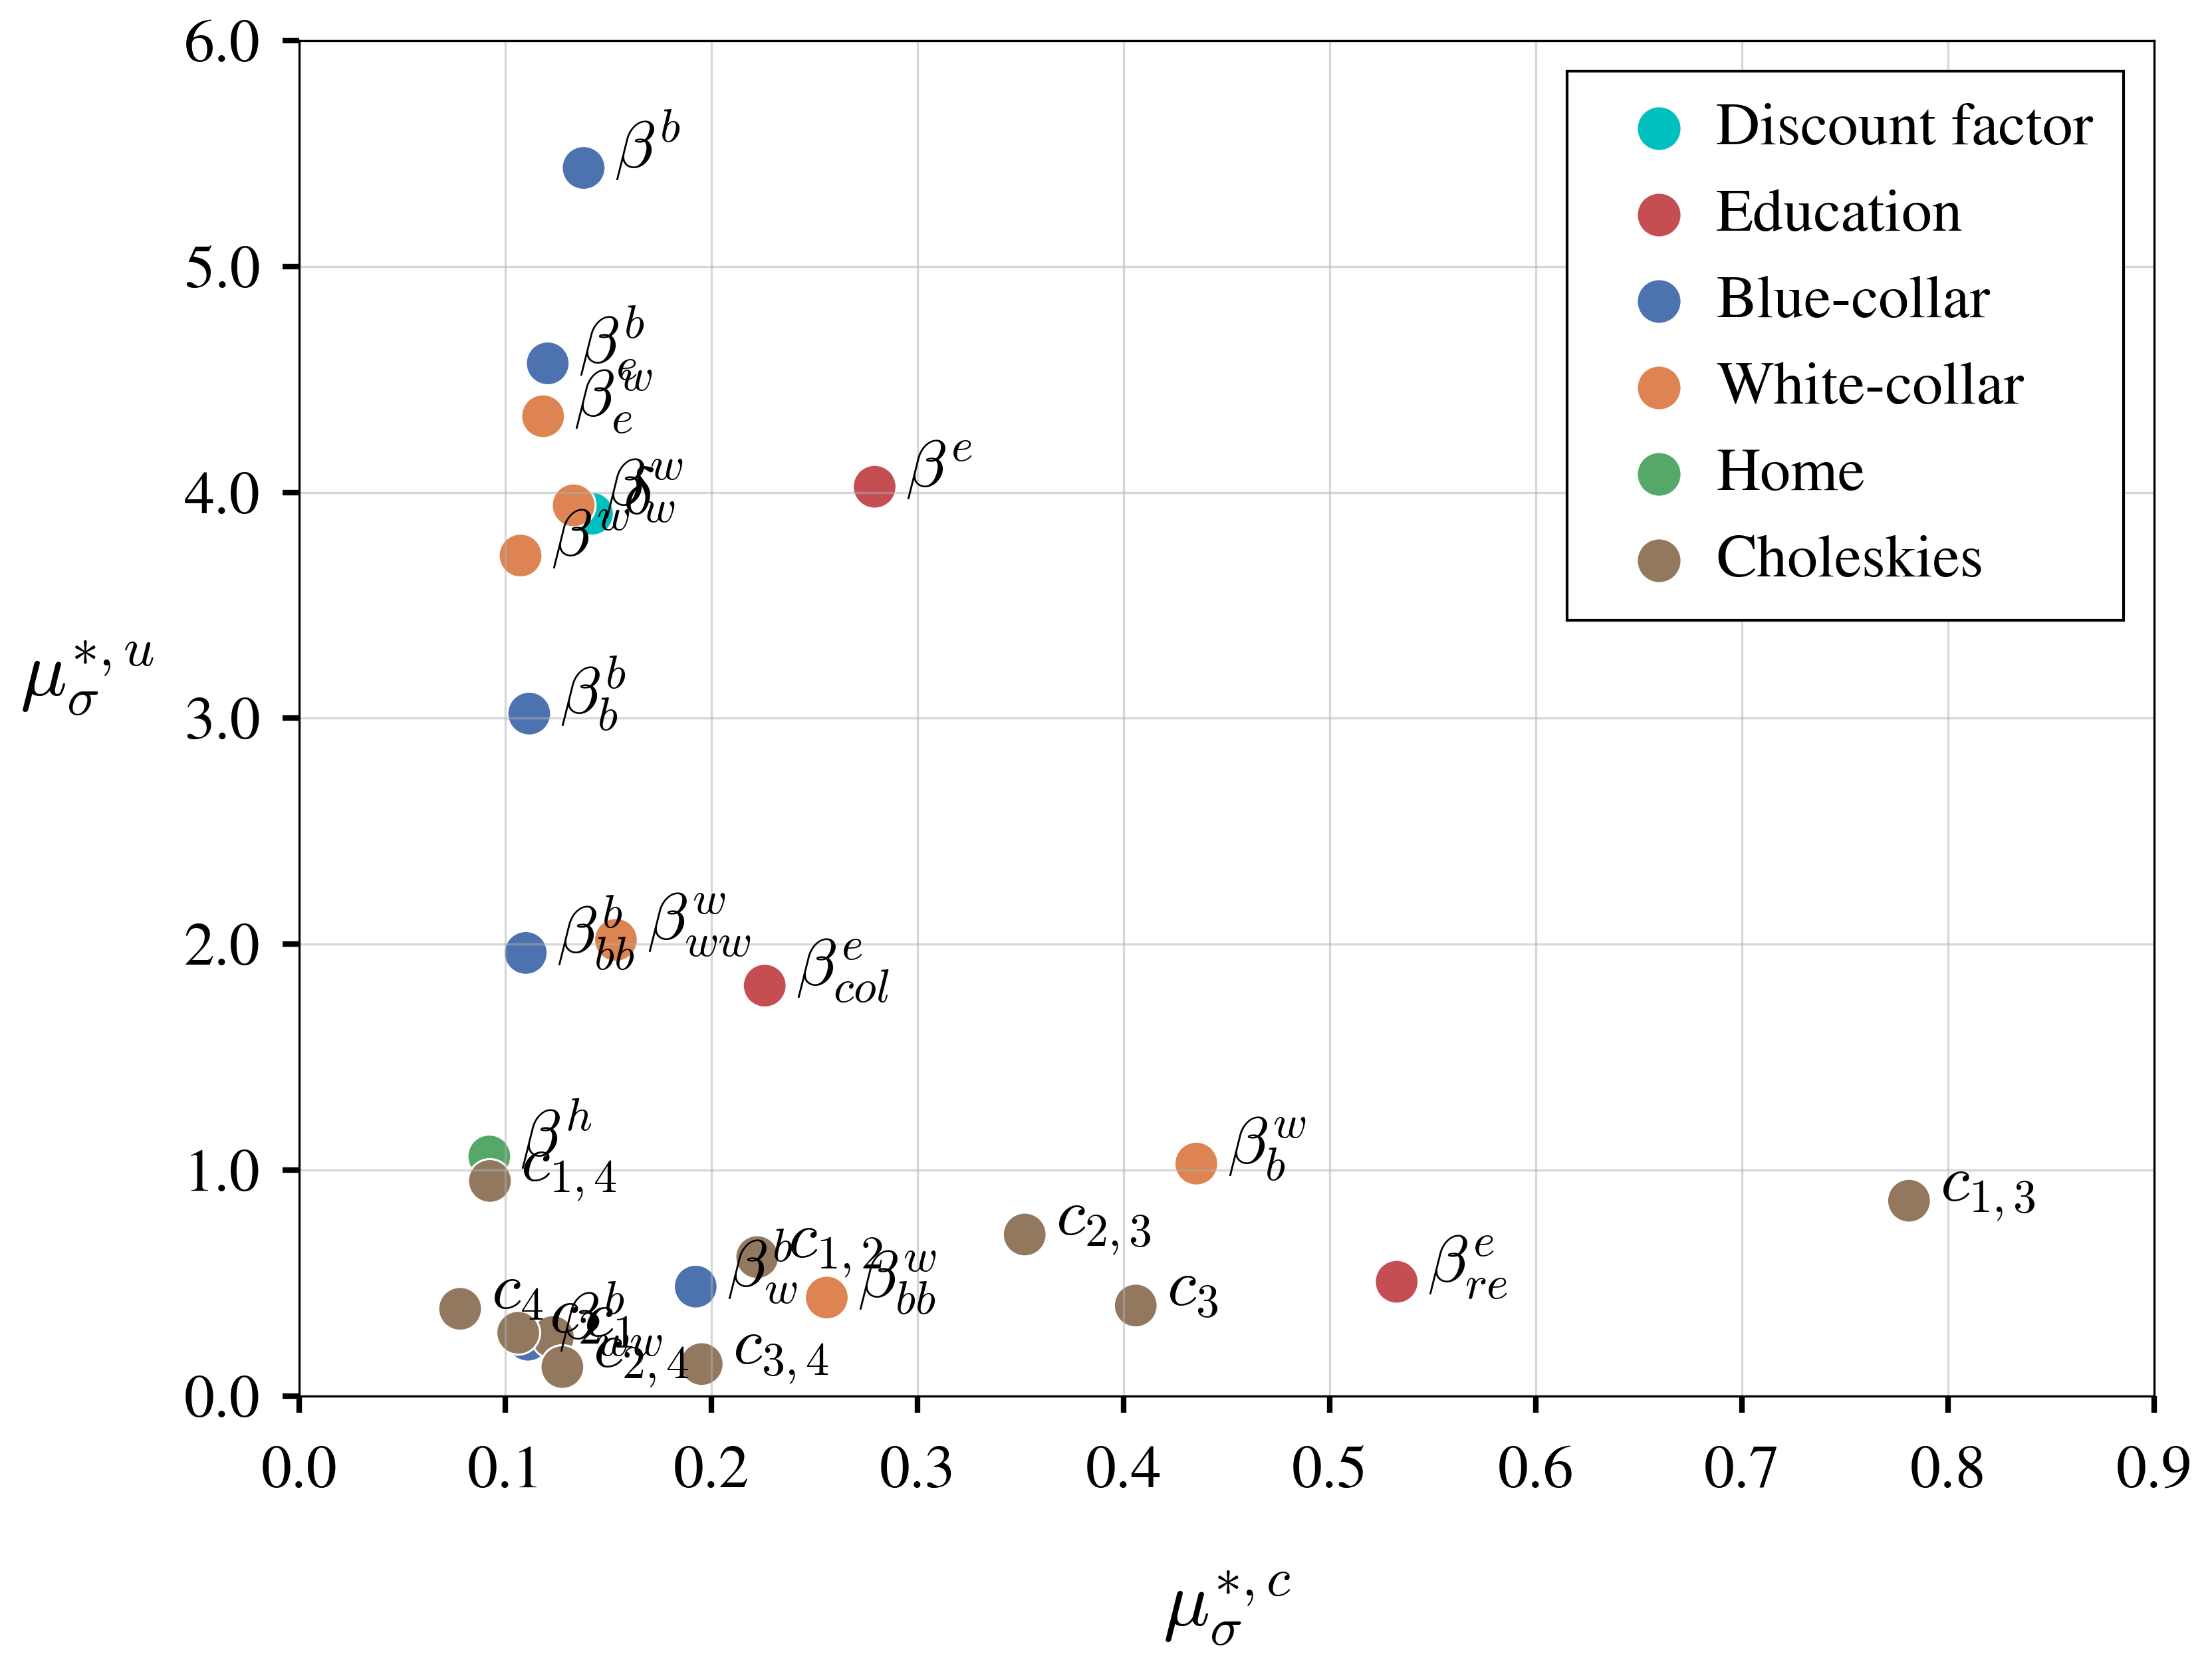
\includegraphics[scale=0.52]{../../../scrypy/figures/scatter_traj}
	\label{fig:traj}
\end{figure}

\begin{figure}[H]
	\caption{Sigma-normalized mean absolute Elementary Effects for radial design}
	\centering
	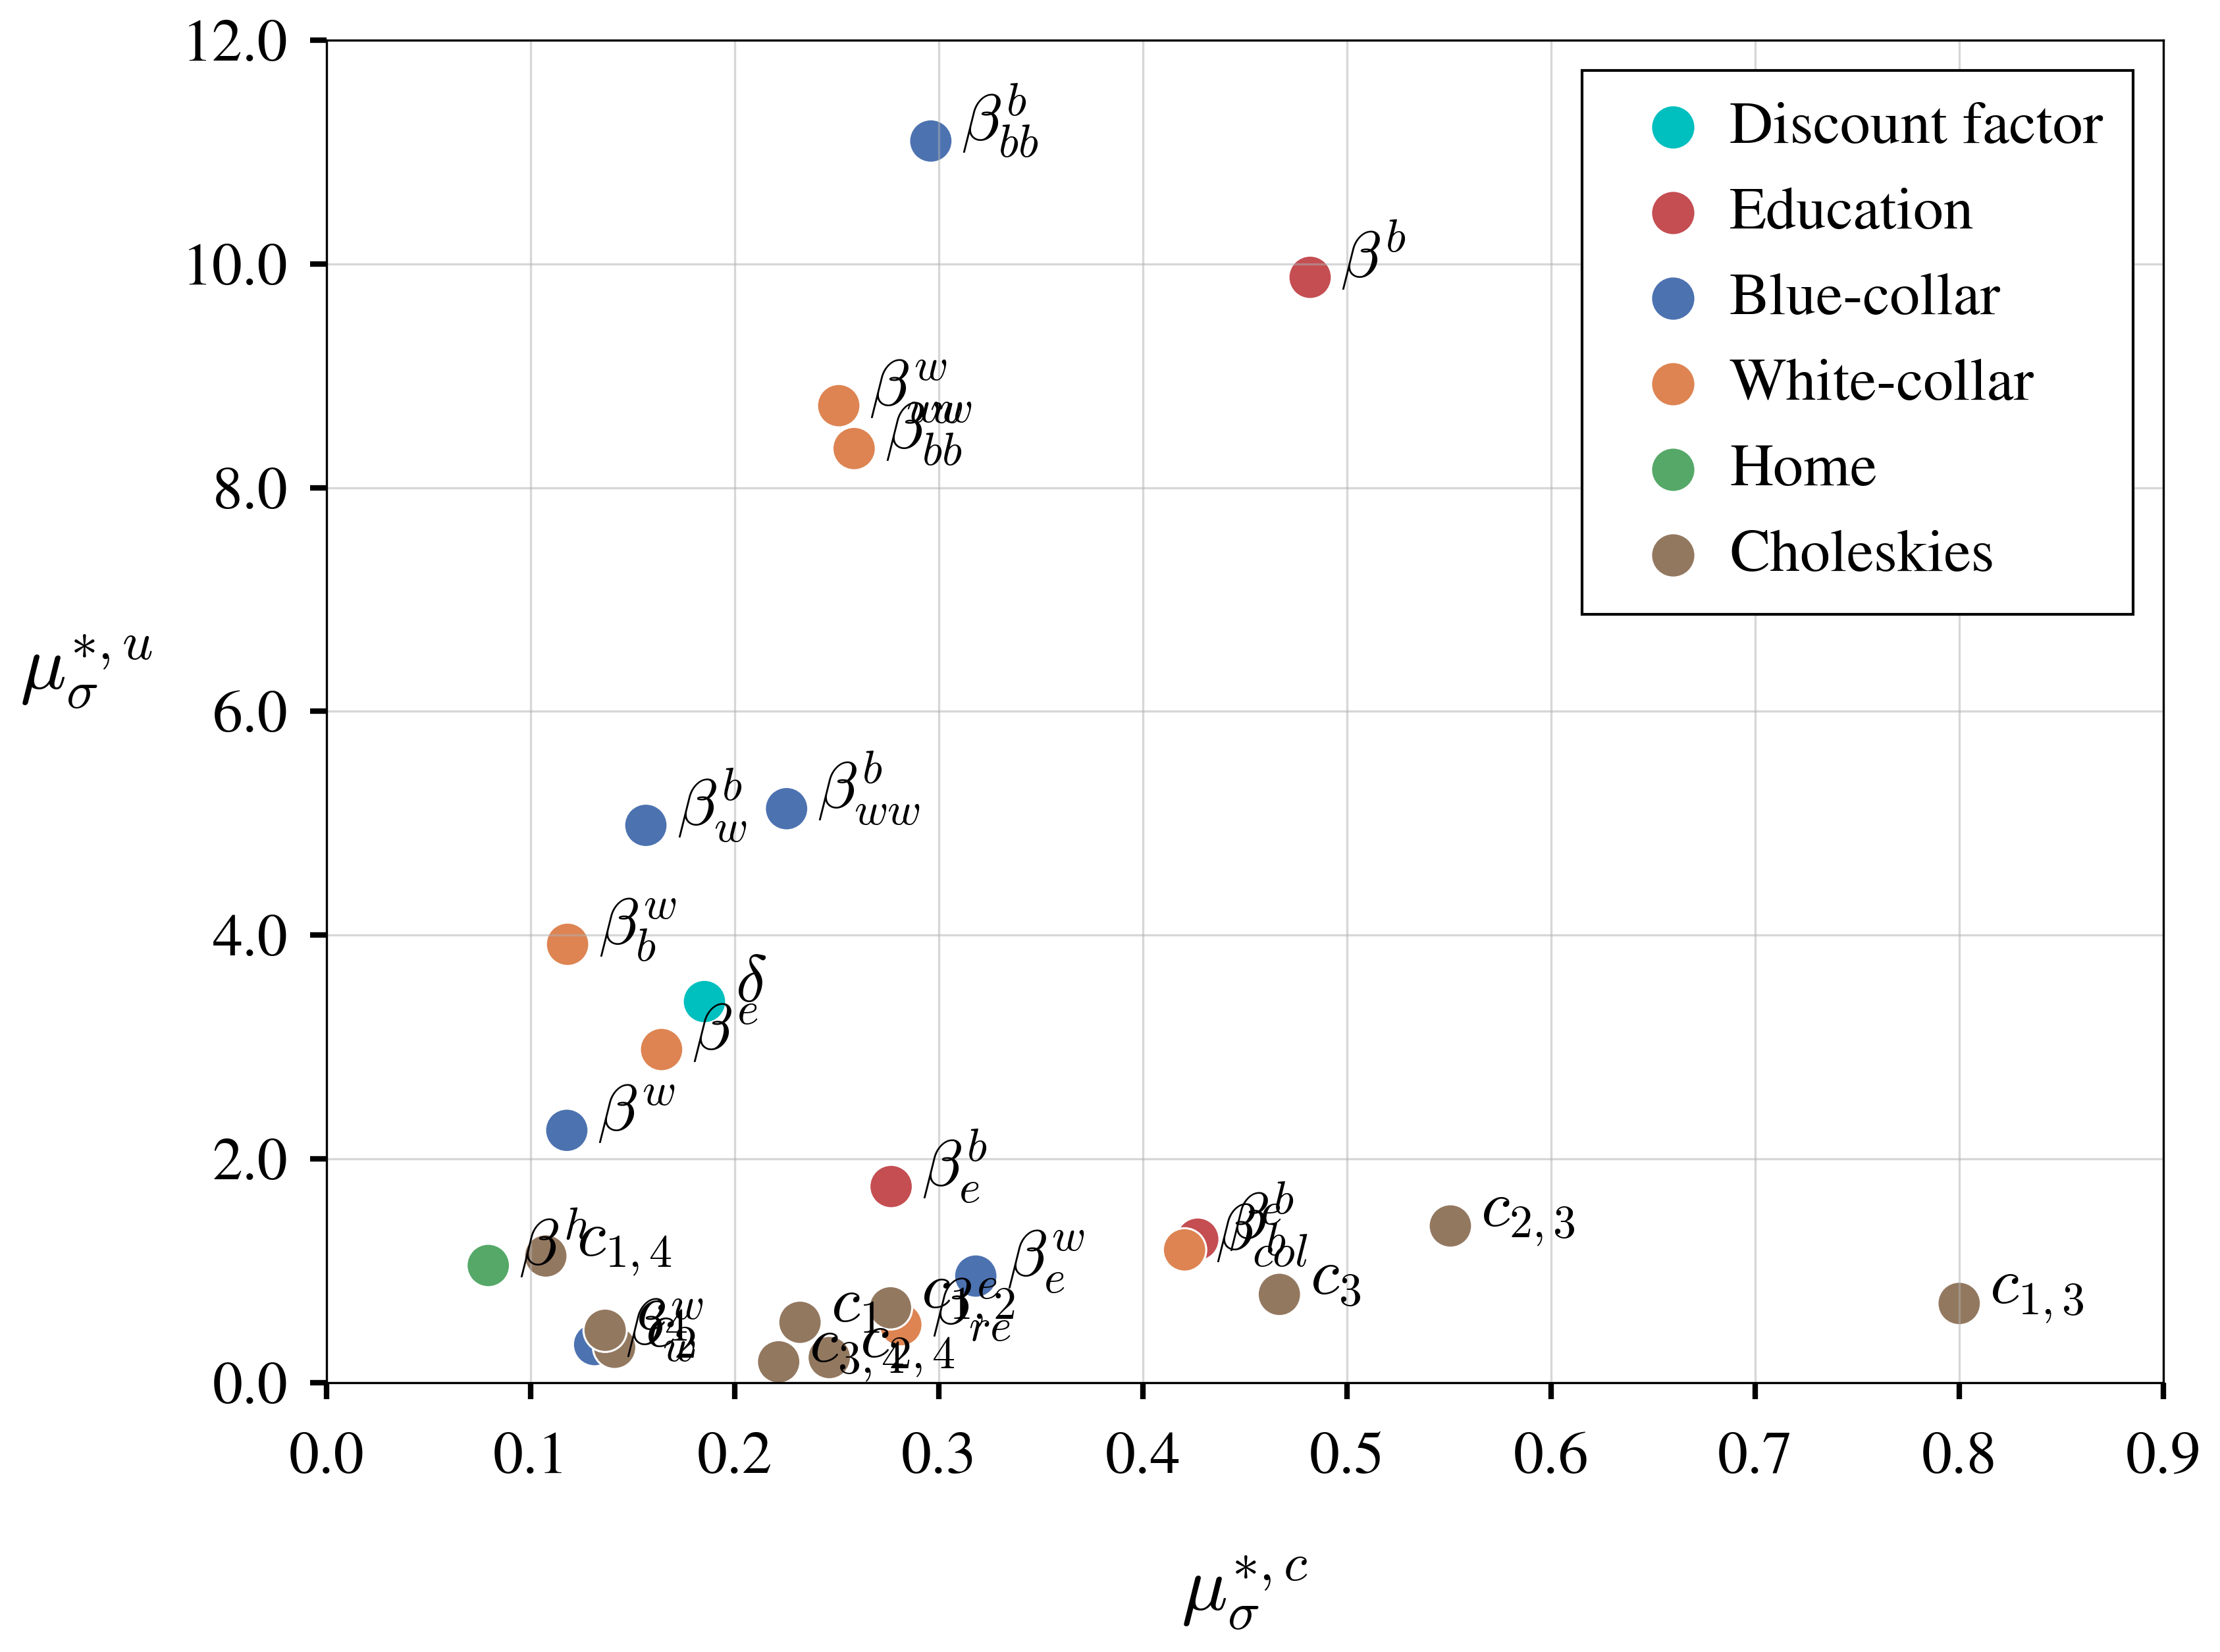
\includegraphics[scale=0.52]{../../../scrypy/figures/scatter_rad}
	\label{fig:rad}
\end{figure}


\newpage
\bibliography{../../bibliography/literature}

\end{document}